\section{数据处理}
\subsection{数据获取}
通过Python爬虫获取了1月20日至今的疫情数据。
此处确诊与重症均为去除死亡人数的数值。
\\
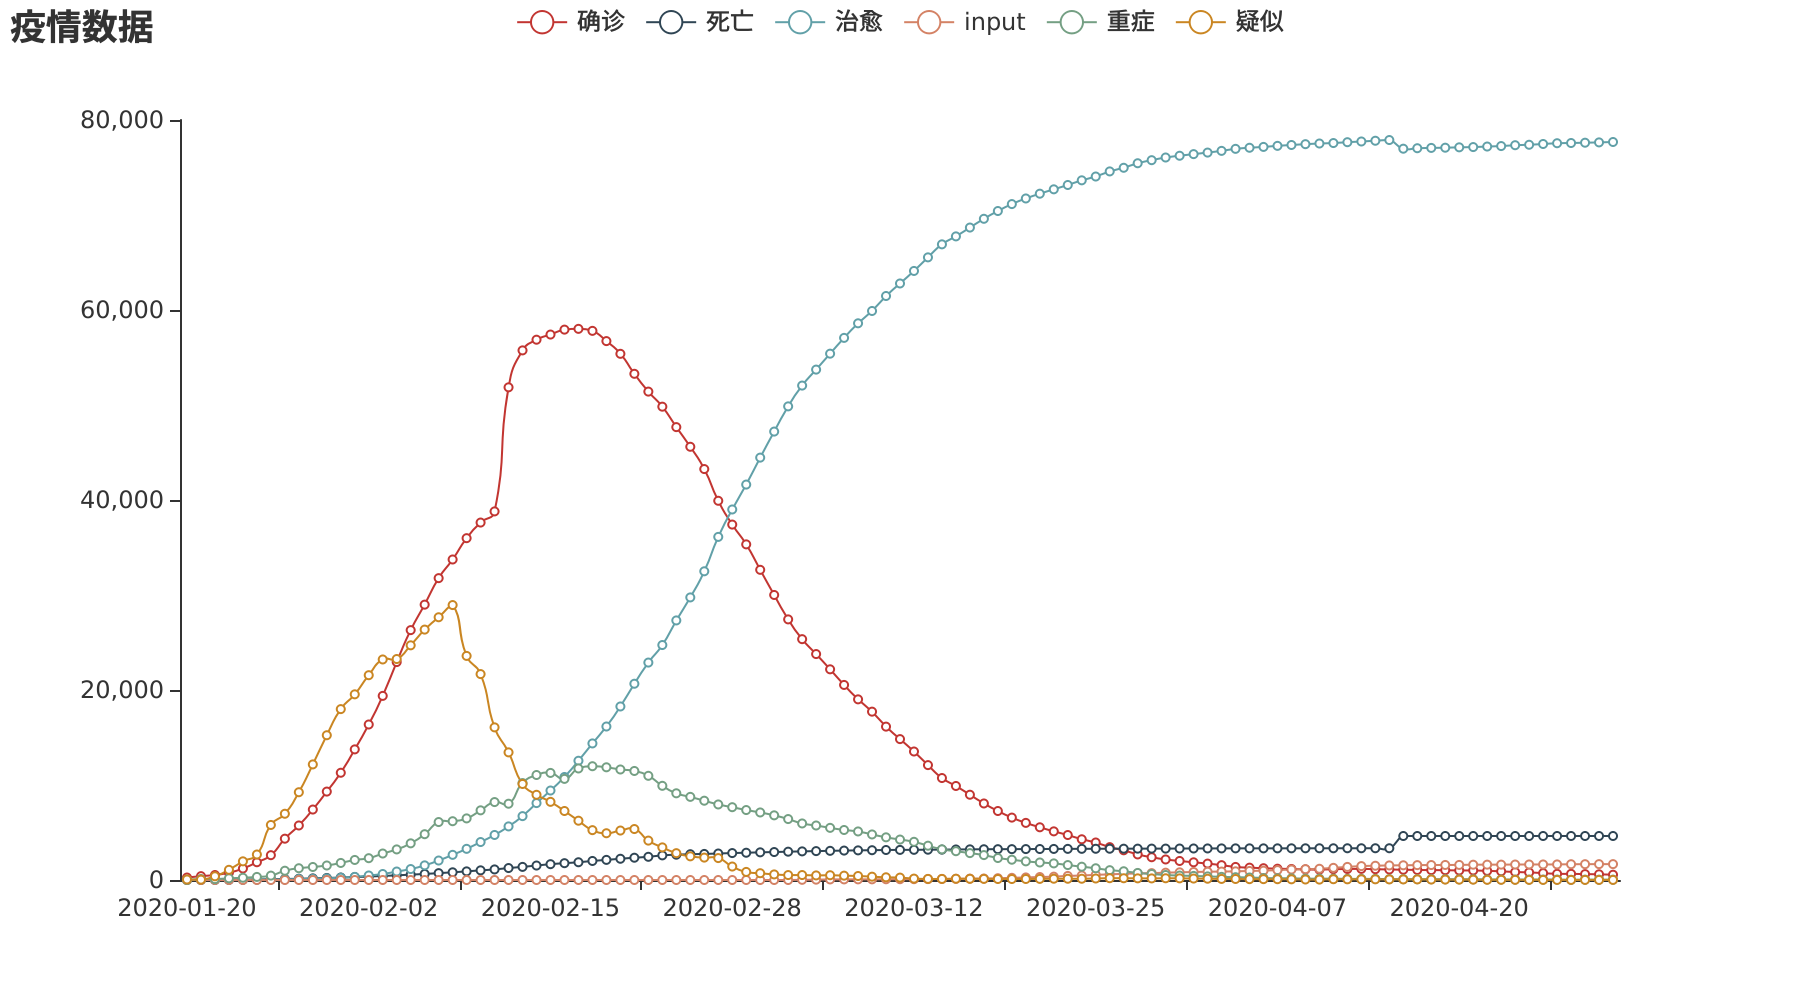
\includegraphics[width=\imagewidth]{疫情数据.png}
\par
可见治愈曲线相较确诊及疑似曲线明显滞后。
\subsection{数据分析}
对数据进行简单的处理,得到每日新增人数曲线。
\\
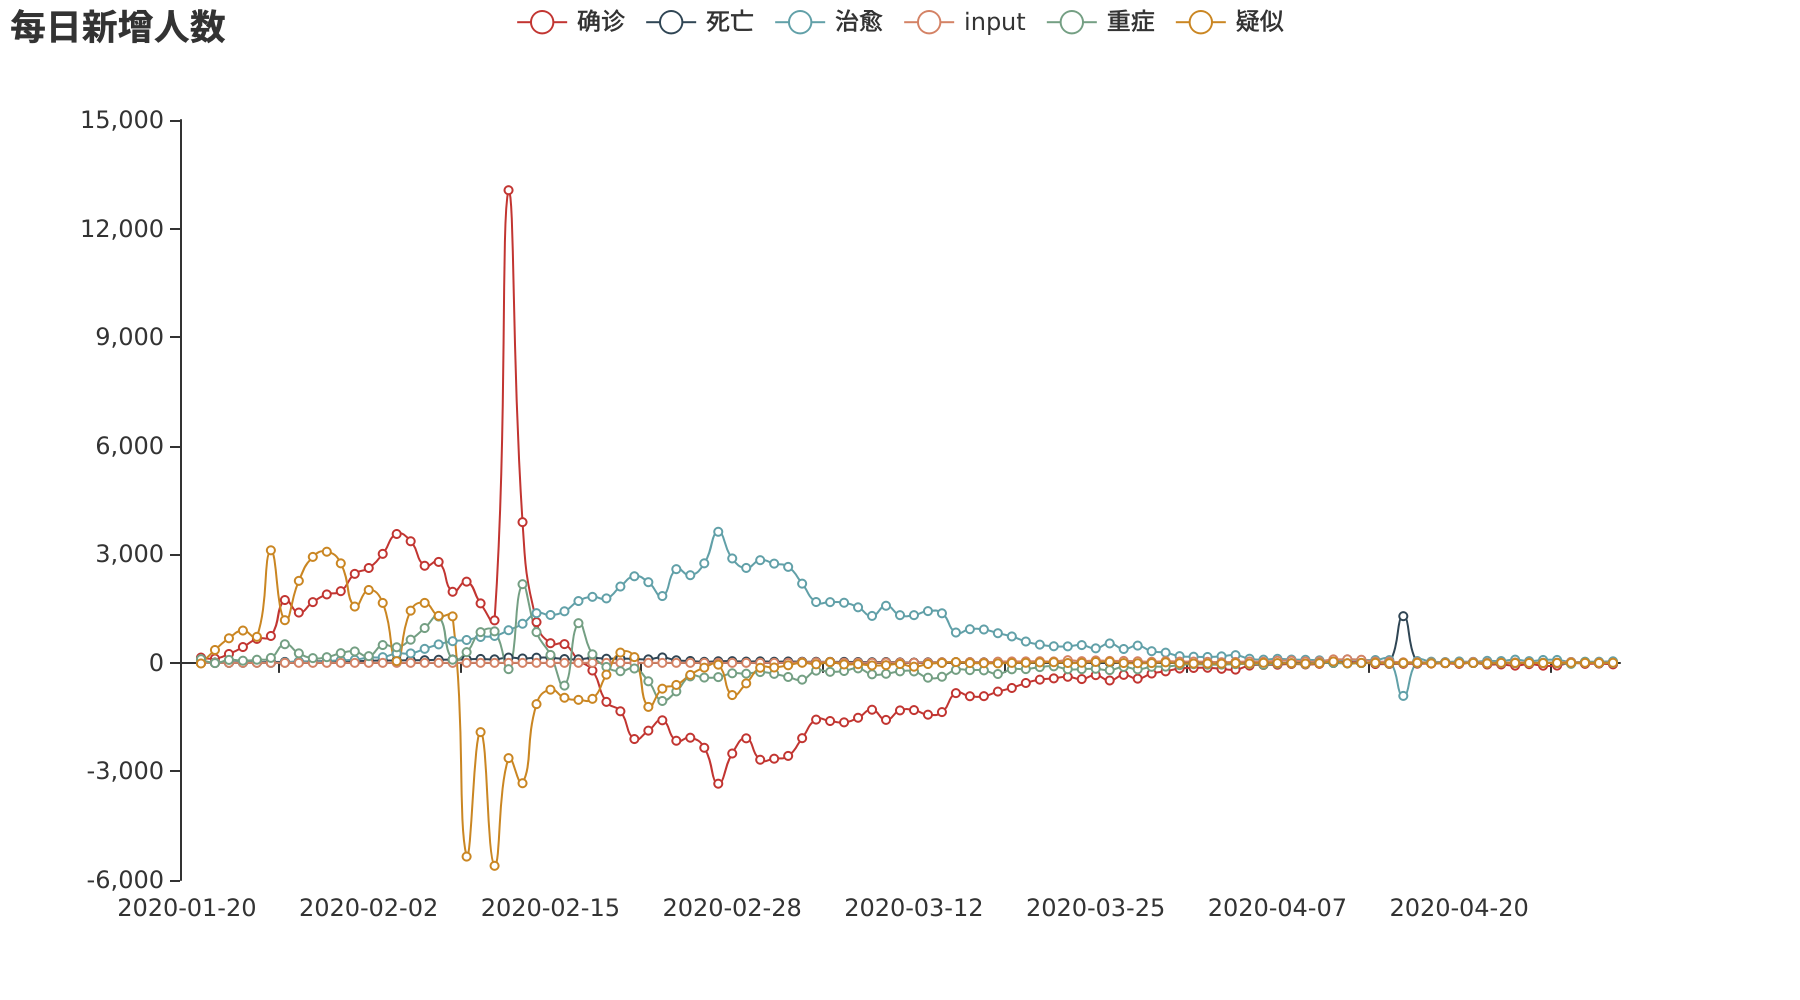
\includegraphics[width=\imagewidth]{每日新增人数.png}
\par
对数据进行简单的观察,可见2月12日确诊人数猛增,
这是因为重新规定了确诊条件,导致许多人被纳入确诊人数。
\par
通过确诊死亡比例可以大致判断致死率。
\\
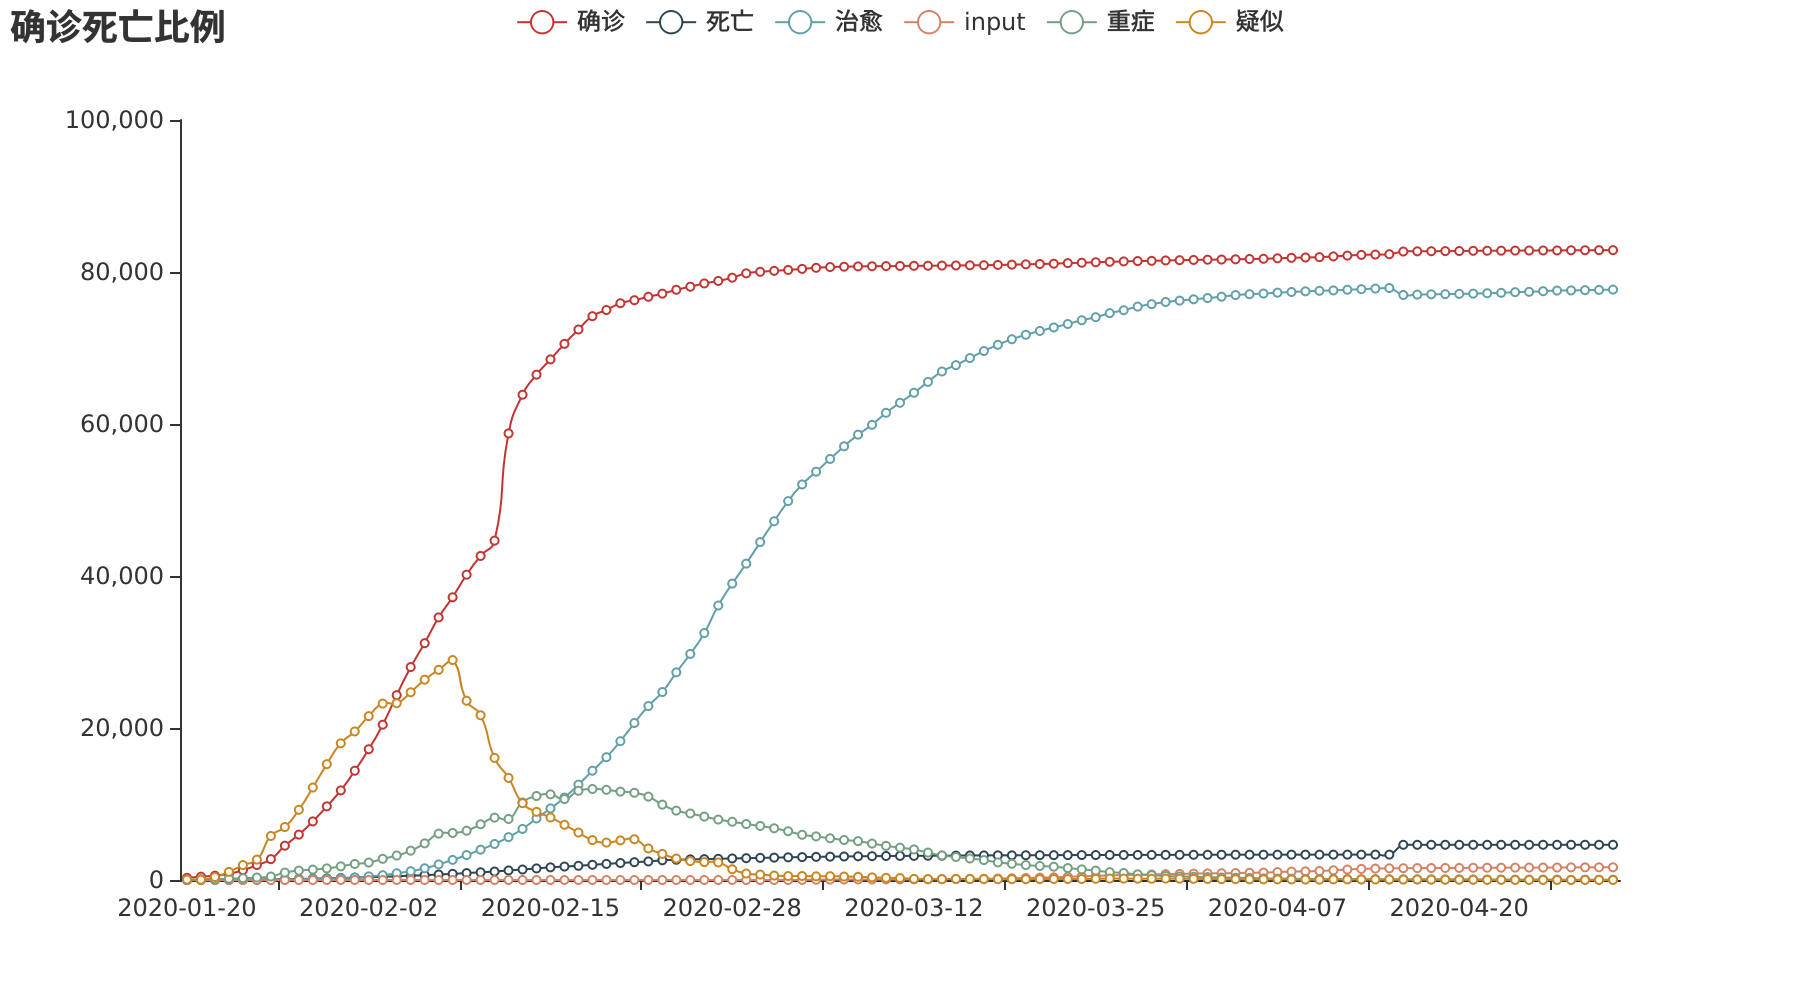
\includegraphics[width=\imagewidth]{确诊死亡比例.png}
\par
可见死亡比例在$0.2\sim 0.5$间波动,最终稳定于$0.5$。
\\
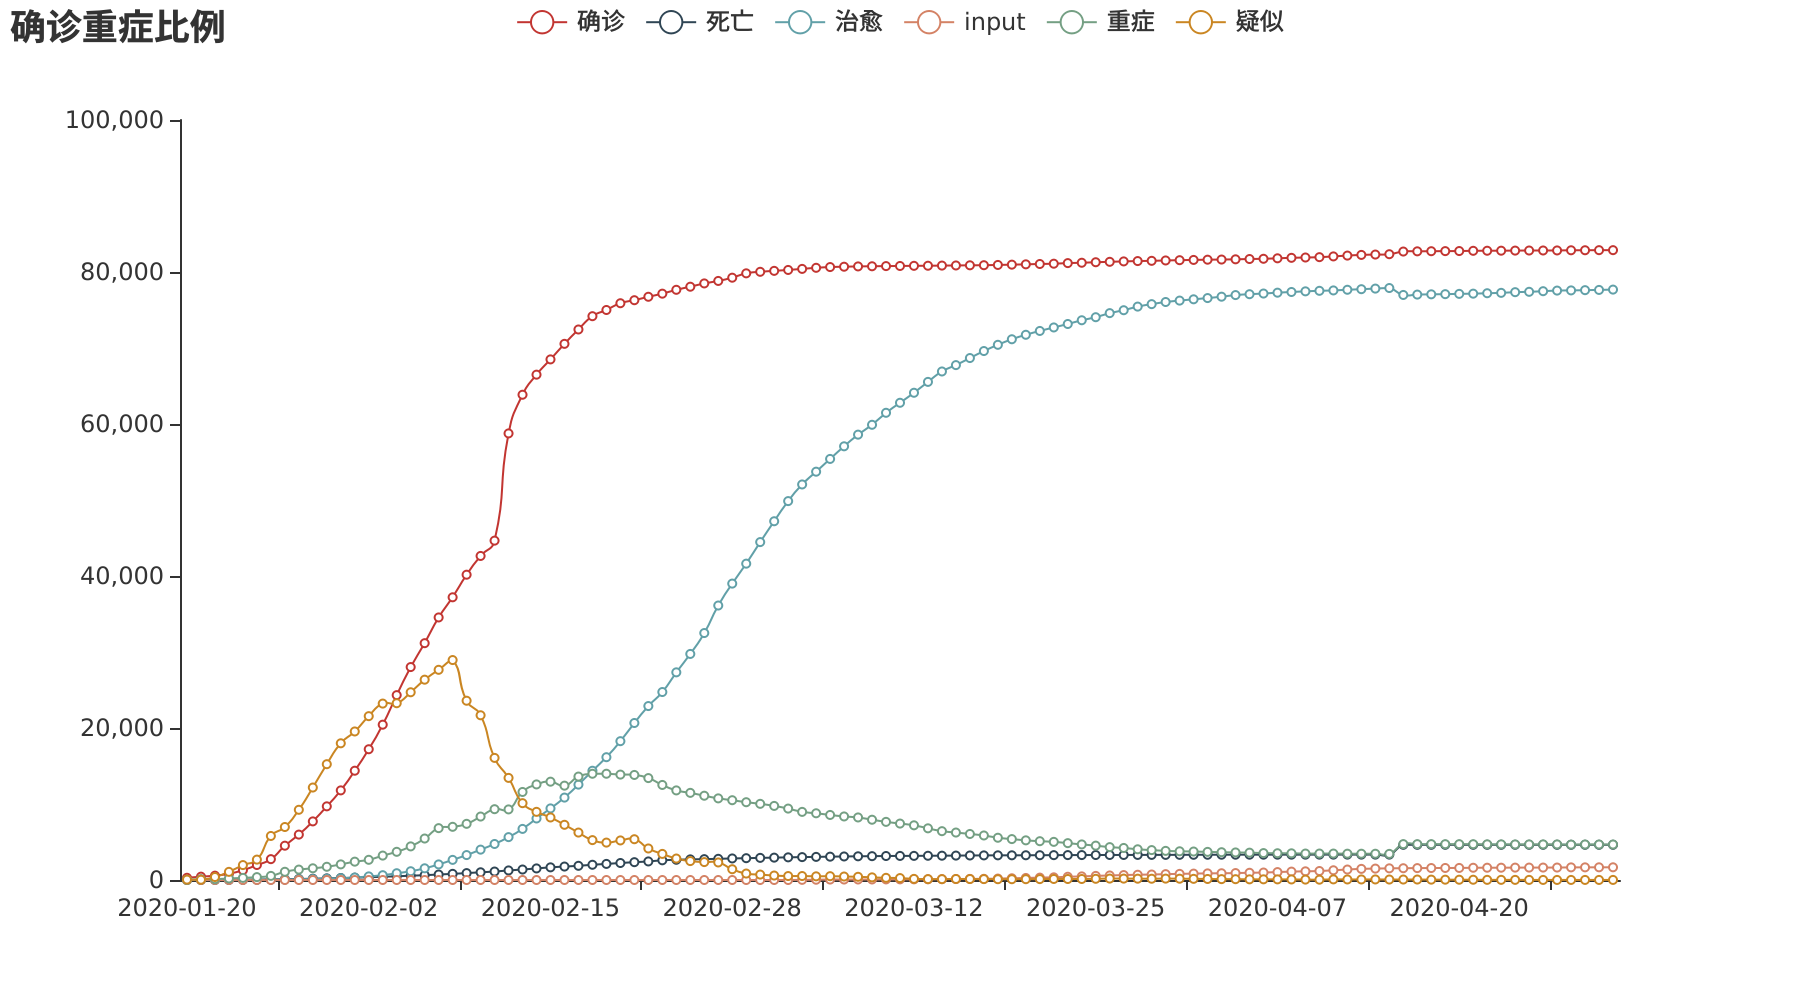
\includegraphics[width=\imagewidth]{确诊重症比例.png}
\par
可知,自2月中旬起,重症比例逐步下降。
\\
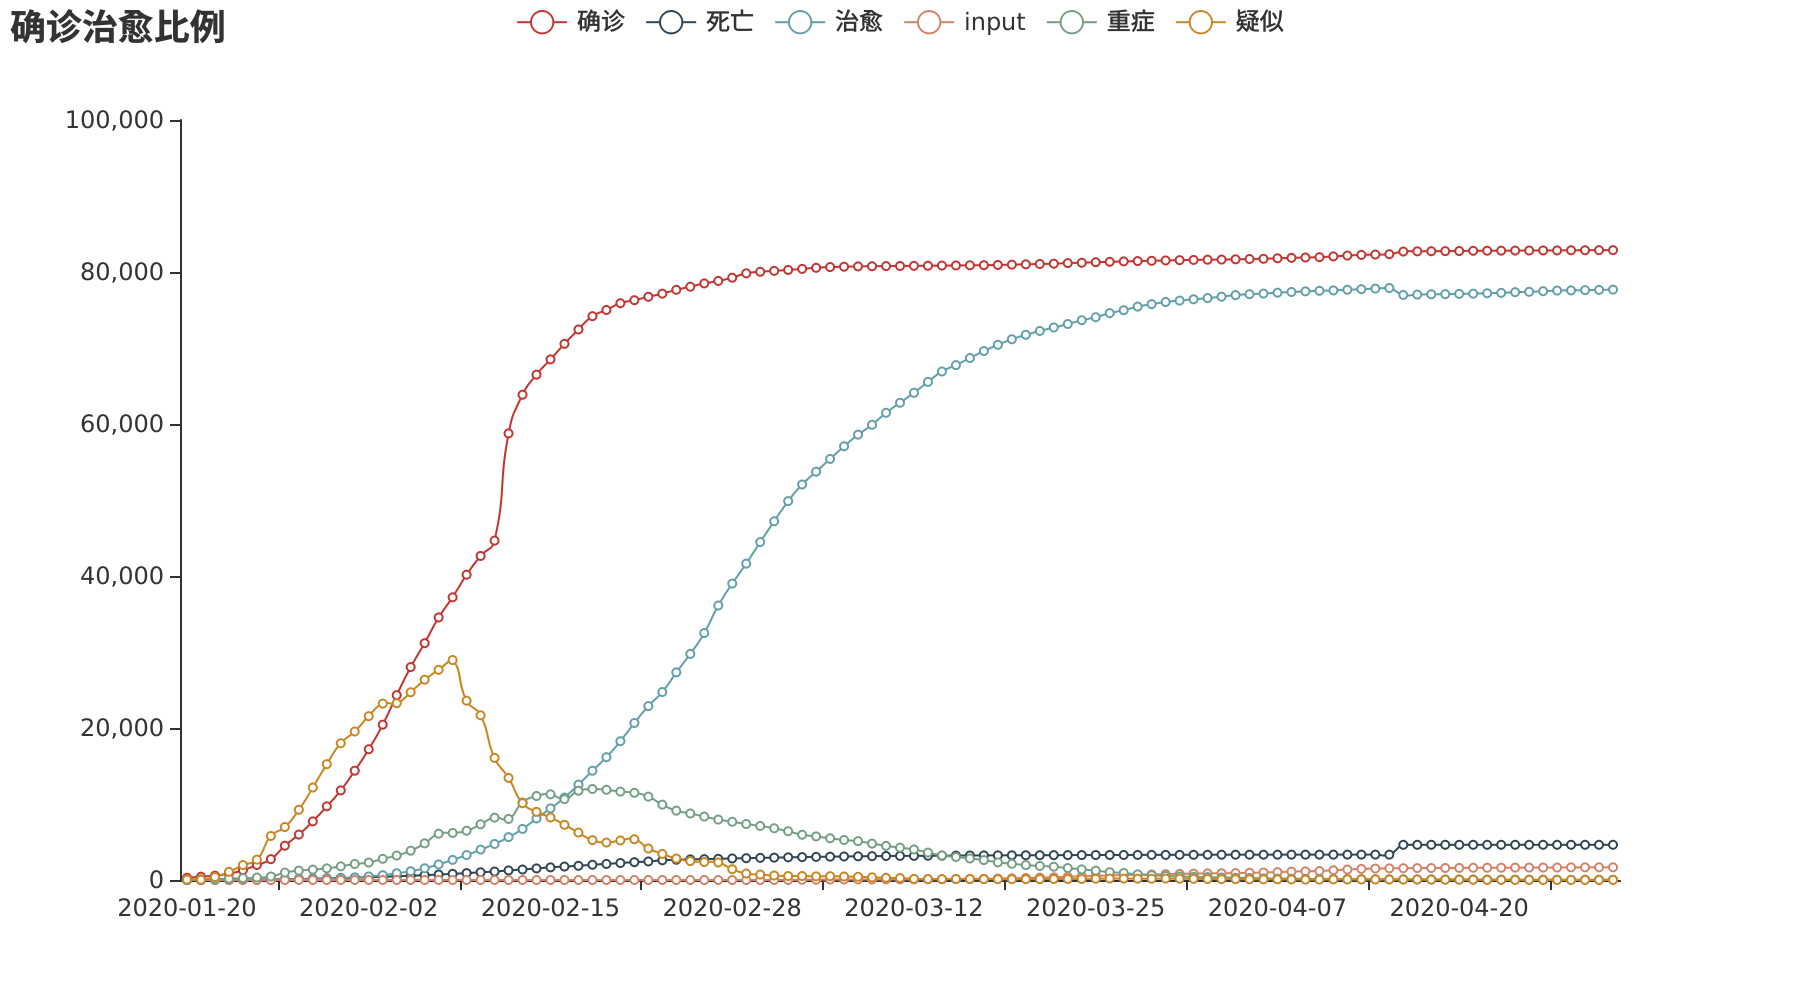
\includegraphics[width=\imagewidth]{确诊治愈比例.png}
\par
可见治愈率越来越高,大体呈$logtic$回归趋势。
\section{数据拟合}
\par
众多学者用不同的方法计算出病毒的基本生殖数等参数\cite{估计2019年新型冠状病毒的流行性:数学建模研究,估计2020年公主邮轮船上2019年新型冠状病毒的无症状比率,协调基本生殖数量及其不确定性的早期暴发估计:新型冠状病毒(SARS-CoV-2)暴发的框架和应用},
本文采用$L-BFGS-B$梯度下降方式进行拟合。
\subsection{拟合结果}
\subsubsection{SIR}
\showfigure{SIR}
\subsubsection{SEIR}
\showfigure{SEIR}
\subsubsection{SEIRD}
\showfigure{SEIRD}
\subsubsection{SEIRS}
\showfigure{SEIRS}
\subsection{考虑隔离因素}
在COVID-19疫情的早期,防护措施较为薄弱,故病毒感染率较高,
而在强有力的隔离措施下,病毒的传染率大幅降低。
王晓红于\citeyear{一类具有潜伏期的SEIR手足口病模型的研究}年将$SEIRS$模型
用于预测手足口病的疫情趋势\cite{一类具有潜伏期的SEIR手足口病模型的研究},
考虑了康复者复发的情况。
隔离措施前后的模型参数都会引起较大变化,
故将其分段处理以2月12日为分界点将其分为两部分对其分别进行模拟。
\subsubsection{SIR}
\showfigures{SIR}
\subsubsection{SEIR}
\showfigures{SEIR}
\subsubsection{SEIRD}
\showfigures{SEIRD}
\subsubsection{SEIRS}
\showfigures{SEIRS}
\subsection{结果评估}